% This is a Basic Assignment Paper but with like Code and stuff allowed in it, there is also url, hyperlinks from contents included. 

\documentclass[openany]{report}

% Preamble

\usepackage[margin=1in]{geometry}
\usepackage{amsfonts, amsmath, amssymb}
\usepackage{fancyhdr, float, graphicx}
\usepackage[utf8]{inputenc} % Required for inputting international characters
\usepackage[T1]{fontenc} % Output font encoding for international characters
\usepackage{fouriernc} % Use the New Century Schoolbook font
\usepackage[nottoc, notlot, notlof]{tocbibind}
\usepackage{listings}
\usepackage{xcolor}
\usepackage{blindtext}
\usepackage{hyperref}
\usepackage{minted}

\hypersetup{
    colorlinks=true,
    linkcolor=black,
    filecolor=magenta,      
    urlcolor=blue,
    pdfpagemode=FullScreen,
    }

\definecolor{codegreen}{rgb}{0,0.6,0}
\definecolor{codegray}{rgb}{0.5,0.5,0.5}
\definecolor{codepurple}{rgb}{0.58,0,0.82}
\definecolor{backcolour}{rgb}{0.95,0.95,0.92}

\lstdefinestyle{mystyle}{
    backgroundcolor=\color{backcolour},   
    commentstyle=\color{codegreen},
    keywordstyle=\color{magenta},
    numberstyle=\tiny\color{codegray},
    stringstyle=\color{codepurple},
    basicstyle=\ttfamily\footnotesize,
    breakatwhitespace=false,         
    breaklines=true,                 
    captionpos=b,                    
    keepspaces=true,                 
    numbers=left,                    
    numbersep=5pt,                  
    showspaces=false,                
    showstringspaces=false,
    showtabs=false,                  
    tabsize=2
}

\lstset{style=mystyle}

% Header and Footer
\pagestyle{fancy}
\fancyhead{}
\fancyfoot{}
\fancyhead[L]{\textit{\Large{Report - 4th Year B. Tech}}}
\fancyhead[R]{\textit{Krishnaraj Thadesar}}
\fancyfoot[C]{\thepage}
\renewcommand{\footrulewidth}{1pt}

% Other Doc Editing
% \parindent 0ex
%\renewcommand{\baselinestretch}{1.5}

\begin{document}

\chapter{Individual Contribution}
\section{Problem Statement}
\section{Student Details}
\textbf{Krishnaraj Thadesar} \\
\textbf{PRN:} 1032210888 \\
\textbf{Roll Number:} 15 \\
\textbf{Panel:} A \\
\section{Module Title}
backend development  jaisa kuch
\begin{figure}[H]
    \centering
    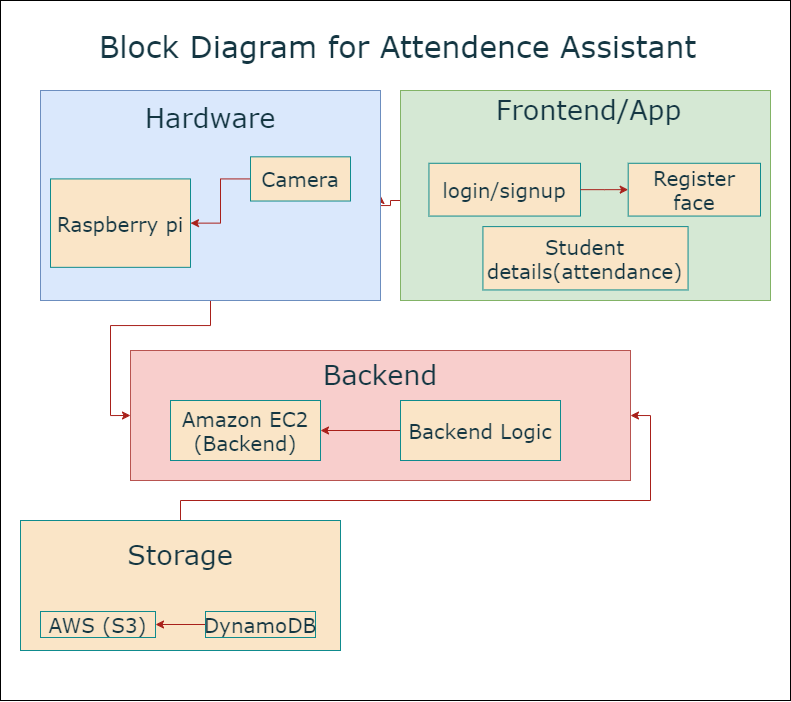
\includegraphics[width=.95\textwidth]{../imgs/block diagram.png}
    \caption{Block Diagram, Individual Contribution has been highlighted for Krishnaraj Thadesar}
    \label{fig:block_diagram}
\end{figure}
\section{Project Module Scope}
backend ka scope pura upar hai iska (current wala change hoga )
\section{Project Modules}
har module me kya contri kiya
1. so like frontend - helped in figma designs
2. backend made api
3. model training hleped in reserarch
4. research for papers etc
5. testing
6. deployment

sab me kya kya kiya thoda achhe se 1 para dal de

% parth
\chapter{Individual Contribution}
\section{Problem Statement}
\section{Student Details}
\textbf{Parth Zarekar} \\
\textbf{PRN:} 1032210888 \\
\textbf{Roll Number:} 15 \\
\textbf{Panel:} A \\
\section{Module Title}
backend development  jaisa kuch
\begin{figure}[H]
    \centering
    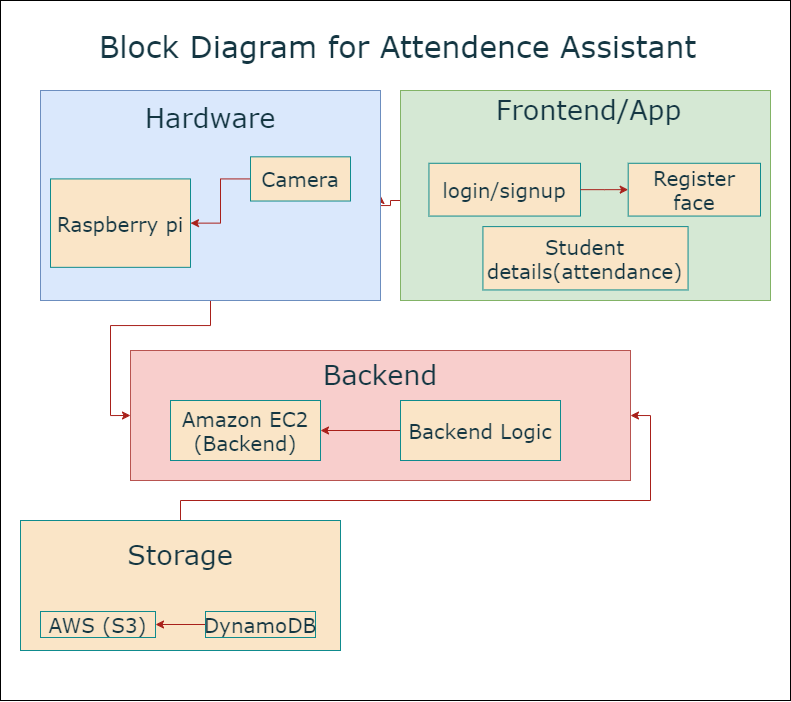
\includegraphics[width=.95\textwidth]{../imgs/block diagram.png}
    \caption{Block Diagram, Individual Contribution has been highlighted for Krishnaraj Thadesar}
    \label{fig:block_diagram}
\end{figure}
\section{Project Module Scope}
backend ka scope pura upar hai iska (current wala change hoga )
\section{Project Modules}
har module me kya contri kiya
1. so like frontend - helped in figma designs
2. backend made api
3. model training hleped in reserarch
4. research for papers etc
5. testing
6. deployment

sab me kya kya kiya thoda achhe se 1 para dal de

% karad
\chapter{Individual Contribution}
\section{Problem Statement}
\section{Student Details}
\textbf{Parth Zarekar} \\
\textbf{PRN:} 1032210888 \\
\textbf{Roll Number:} 15 \\
\textbf{Panel:} A \\
\section{Module Title}
backend development  jaisa kuch
\begin{figure}[H]
    \centering
    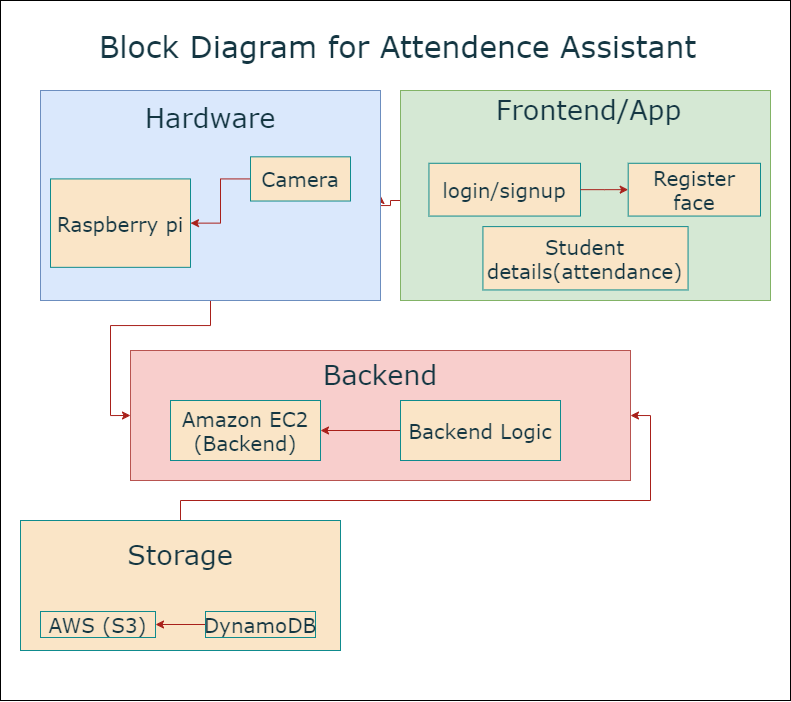
\includegraphics[width=.95\textwidth]{../imgs/block diagram.png}
    \caption{Block Diagram, Individual Contribution has been highlighted for Krishnaraj Thadesar}
    \label{fig:block_diagram}
\end{figure}
\section{Project Module Scope}
backend ka scope pura upar hai iska (current wala change hoga )
\section{Project Modules}
har module me kya contri kiya
1. so like frontend - helped in figma designs
2. backend made api
3. model training hleped in reserarch
4. research for papers etc
5. testing
6. deployment

sab me kya kya kiya thoda achhe se 1 para dal de

% saubhagya

\chapter{Individual Contribution}
\section{Problem Statement}
\section{Student Details}
\textbf{Parth Zarekar} \\
\textbf{PRN:} 1032210888 \\
\textbf{Roll Number:} 15 \\
\textbf{Panel:} A \\
\section{Module Title}
backend development  jaisa kuch
\begin{figure}[H]
    \centering
    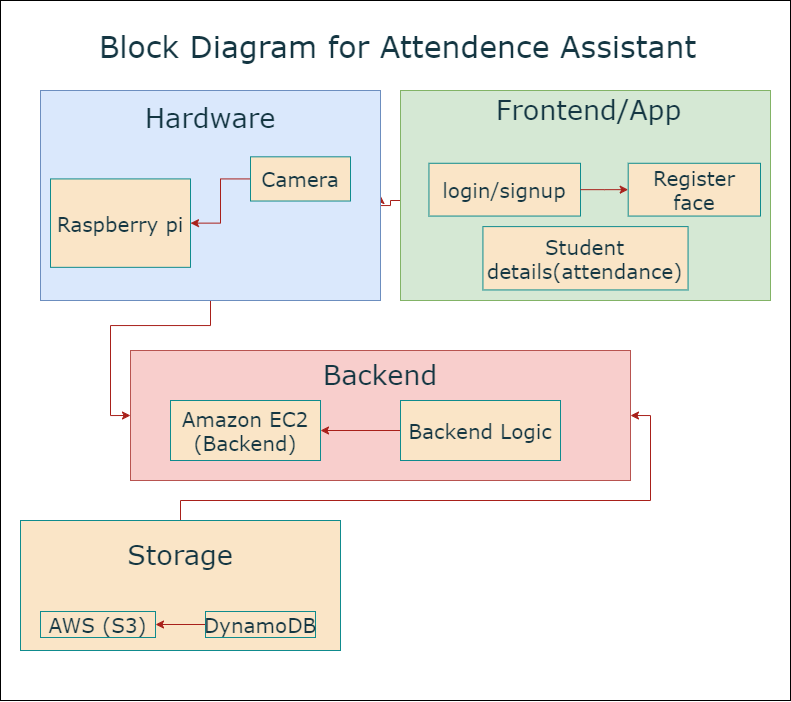
\includegraphics[width=.95\textwidth]{../imgs/block diagram.png}
    \caption{Block Diagram, Individual Contribution has been highlighted for Krishnaraj Thadesar}
    \label{fig:block_diagram}
\end{figure}
\section{Project Module Scope}
backend ka scope pura upar hai iska (current wala change hoga )
\section{Project Modules}
har module me kya contri kiya
1. so like frontend - helped in figma designs
2. backend made api
3. model training hleped in reserarch
4. research for papers etc
5. testing
6. deployment

sab me kya kya kiya thoda achhe se 1 para dal de

\end{document}
